%%%%%%%%%%%%%%% Implementation %%%%%%%%%%%%%%%%%%%%%%%%%
\section{Implementation}
\label{sec:implementation}

In this section we will describe some of the most important implementation
details that were undertaken during the development phase.

\subsection{Creating and deploying a bundle}
\label{subsec:creating-bundles}

In this section we will enumerate the necessary steps to create
an OSGi bundle and deploy it in the Knopflerfish framework, assuming we have 
already set up the necessary tools (Eclipse, Knopflerfish eclipse plugin, etc)
\footnote{Details about the tools can be found in Section \ref{sec:tools}.}.
It is based on the tutorials in \cite{osgi-tutorial} and \cite{osgi09}.


\subsubsection{Creating the project and the manifest}
First of all, we need to create an OSGi project and ensure that the
\verb|framework.jar| file is imported in the Java Build Path, otherwise we will
not be able to access the OSGi classes and interfaces provided by Knopflerfish.
\newline
One of the differences with respect to a common Java project is the need of
defining a manifest file which contains the description of the bundle. This
manifest is used by the framework to get information about it and to deploy it
successfully. 
As an example we show a simplified version of \verb|RepositoryManager|`s
manifest:

\verbatiminput{code/repository_manifest}

From which we can remark the following attributes:
\begin{itemize}
  \item Export-Packages: It informs the framework which are the classes and
  interfaces offered by this bundle.
  \item Bundle-Classpath: It is necessary to establish all the external
  libraries used by this bundle.
  \item Bundle-Activator: It tells the framework which class is the
  \verb|Activator| class, it is a similar concept to the ``main" class in a
  normal Java application.
  \item Import-Package: It informs the framework about the bundles it needs to
  have access to (only locals). 
\end{itemize}

Appendix \ref{appendix:manifests} contains all the manifests from all the
bundles developed for this project.
\newline
It is also necessary to create an Ant Build file to build the project, but
assuming we are using OSGi Knopflefish plugin for Eclipse, it is created
automatically.

\subsubsection{Creating an activator}

The next step consists of defining the \verb|Activator| class, a class that
implements the \verb|BundleActivator| interface. This interface requires the
implementation of two methods, \verb|start()| and \verb|stop()|, which are used
by the framework to manage the bundle.
The \verb|start()| and \verb|stop()| methods receive a \verb|BundleContext|
object. We have to store this object once we get it and set the reference back
to \verb|null| when the bundle is stopped. That way, the Garbage Collector can
do its work and free unused resources.
\newline
We have also to register the services by calling the \verb|registerService()|
method of the \verb|BundleContext|. It receives three parameters: the first
parameter is the name of the service interface. The second is the service 
implementation. The third parameter can be used to supply additional 
information about the service as key/value pairs.

As an example, Figure \ref{img:repository-activator} shows
\verb|RepositoryManager|'s activator code.

\begin{figure}[h!]
 \begin{center}

 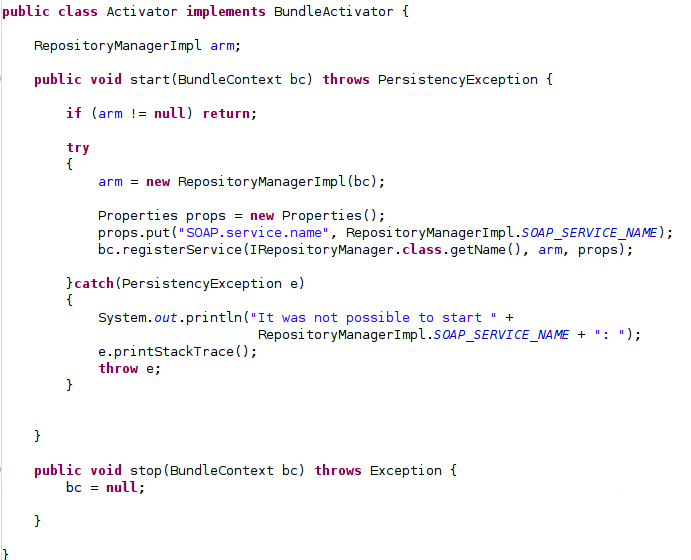
\includegraphics[scale=0.65]{screenshots/repository-activator.png}
  \caption{\label{img:repository-activator}RepositoryManager's activator}
 \end{center}
\end{figure}


\subsubsection{Running the bundles}
Finally, we just need to configure the running configuration. An easy way to
do it is by creating a OSGi run configuration, where we can set the framework,
configure the system properties, etc.
The most delicate part consists of defining the priorities to run the bundles.
This can be problematic for those bundles that make use of other bundles
services when they are run for the first time\footnote{An alternative consists
of creating a \texttt{ServiceTracker} object, but this is out of the scope of
this explanation.}, i.e: the need of \verb|RepositoryManager| to access the
database using \verb|PersistencyManager|'s services when is started for the first time.
\newline
The Figure \ref{img:screenshot-bundles-priorities} shows a screenshot where
the bundles priorities are configured using the OSGi Eclipse plugin.
The configurations for running an ASTRA Node and the ASTRA Backend are
explained in Appendix \ref{appendix:osgi-bundles-config}.

\begin{figure}[h!]
 \begin{center}
 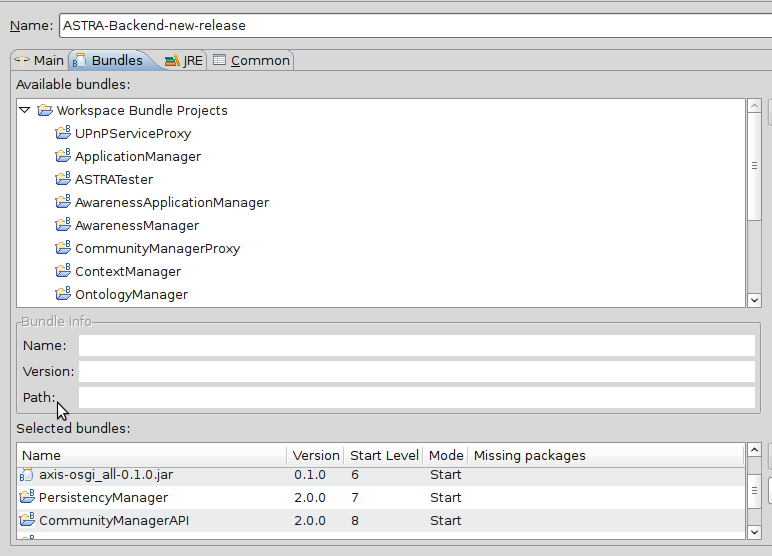
\includegraphics[scale=0.4]{screenshots/back-end-config.png}
  \caption{\label{img:screenshot-bundles-priorities}Bundles priorities
  configuration}
 \end{center}
\end{figure}

After all these steps our bundle can be successfully run and debugged.

\subsection{Implementing MVC in a SWING application}
\label{subsec:implementation-mvc-swing}
In this section we will explain the process carried on to develop the
\verb|ApplicationManager| GUI (whose design was discussed in Section
\ref{subsec:am-design}) following a MVC architectural pattern.
\newline
It is based in some of the ideas explained in \cite{mvc-java} and
\cite{interfaces05}.
\newline
We will summarize it describing the responsibilities of each sub-component:
\begin{itemize}
  \item Controller: It is implemented in a singleton class, which
  	\begin{itemize}
	  \item Keeps track of the user interface components.
	  \item Provides a set of methods that can be called by the events handlers. 
	\end{itemize}
  \item View: All the windows were designed graphically, using a free software
	  plugin for Eclipse called ``Visual Swing 4 Eclipse"\footnote{More details can
	  be found in Section \ref{sec:tools}.}. It offers also facilities to create ``empty"
	  methods that handle the events. This makes the development faster since we
	  only have to:
  	\begin{itemize}
        \item Set the references to the components in the controller.
        \item Establish a relationship between the proper event and the method
        to be called in the controller.
     \end{itemize}
  \item Model: Implements the ``business logic'' that, taking into account the
  SOA nature of the whole project, consists of:
  	\begin{itemize}
        \item Store the user session information and the references to the rest
        of the bundles.
        \item Provides a set of methods with the proper information to be
        consumed by the controller, and make use of the services offered by
        other bundles when necessary.
     \end{itemize}

\end{itemize}

As it was briefly discussed in Section \ref{subsec:am-design}, we assure a
loose coupling relationship between the subcomponents thanks to it.

It is also interesting to remark that the GUI creates background threads to
perform time-consuming tasks, by extending the \verb|SwingWorker| class in
order to keep the GUI responsive \cite{swing-concurrency}. Concretely, threads 
are created for loading the tree hierarchy for remote and local applications.

\subsection{Search engine development}
\label{subsec:implementation-search-engine}
In order to accomplish the requirements related to searching capabilities
(see Section \ref{sec:requirements}) which are captured in Section 
\ref{subsec:searching-use-cases}, we decided to use the open source library
Lucene (see \ref{sec:tech-lucene}).
\newline
Lucene allowed us to provide search capabilities in a really flexible and
powerful way. In this section we will explain the steps we took to create and
integrate the search engine based on this library into \verb|RepositoryManager|
(see Section \ref{subsec:repository-design}).

\subsubsection{Creating the index}
The first step consisted of deciding how the index is going to be created.
\newline
Lucene stores the index in a directory which can be of two different types:
\verb|FSDirectory|, storing the contents in the contents in the file system, or
\verb|RAMDirectory|, storing the contents in memory. Our search engine uses
the latter, since we do not need persistence of this index once 
\verb|RepositoryManager| is stopped, and it offers a better performance.
\newline

Lucene defines a \verb|Document| as the basic unit to be indexed. Every document
is composed of \verb|Fields|, which represent all the information associated to
the \verb|Document|. In our case the notion of what a \verb|Document| is seems
straight: an application, but deciding what information to store about it (the
\verb|Fields|) requires more caution.
\newline
Lucene allows to customize the type of field by configuring how the field is
going to be stored (see Table \ref{table:lucene-storage}) and how is going to
be indexed (see Table \ref{table:lucene-indexation}).

\begin{table}[h!]
	\small
    \begin{center}
		\begin{tabular}{||l|l||}
        
		\hline \hline
		\multicolumn{2}{||c||}{\bfseries{Type of storage}} \\
		\hline
		\hline 
			Type & Description \\
		\hline \hline
			Compress &  Store the original field value in the index in a compressed form.\\
			\hline
			Yes &  Do not store the field value in the index. \\
			\hline
			No & Store the original field value in the index. \\
		\hline \hline

		\end{tabular}
		\caption{\label{table:lucene-storage} Types of field storage options in
		Lucene}
	\end{center}
\end{table}


\begin{table}[h!]
	\small
    \begin{center}
		\begin{tabular}{||l|l|||}
        
		\hline \hline
		\multicolumn{2}{||c||}{\bfseries{Type of indexation}} \\
		\hline
		\hline 
			Type & Description \\
		\hline \hline
			No &  Do not index the field value.\\
			\hline
			Analyzed &  Index the tokens produced by running the field's value through
			an Analyzer.\\
			\hline
			Not Analyzed & Index the field's value without using an Analyzer, so it can
			be searched.\\
			\hline \hline

		\end{tabular}
		\caption{\label{table:lucene-indexation} Types of field indexation in Lucene}
	\end{center}
\end{table}


Taking into account these field types, the Table
\ref{table:lucene-se-fields} summarizes the type of fields we decided to use
and a brief description with the reasons.

\begin{table}[h!]
	\small
    \begin{center}
		\begin{tabular}{||l|l|l|l||}
        
		\hline \hline
		\multicolumn{4}{||c||}{\bfseries{Search engine - fields}} \\
		\hline
		\hline 
			Field & Storage & Indexation & Description\\
		\hline \hline
			App. identifier &  Yes & Not Analyzed & Necessary to return as a result of a
			query.\\
			\hline
			App. description &  Yes & Analyzed & Used for querying.\\
			\hline
			App. type &  Yes & Not Analyzed & Used for querying.\\
			\hline
			App. owner &  Yes & Not Analyzed & Used to filter applications which belong
			to \\
			 & & & the user who is performing the query\\
			\hline
			App. tags &  Yes & Analyzed & Used for querying.\\
			\hline
			\hline

		\end{tabular}
		\caption{\label{table:lucene-se-fields} Fields used by RepositoryManager's
		search engine index}
	\end{center}
\end{table}

The reason why we need to store all the fields is based on the lack of
functionalities to update the document fields in the index. Our search engine
needs to take into account the addition and removal of some fields associated
to a document dynamically (i.e.: the tags which are added or removed), therefore
we need to update that document in the index. The only way to implement this in the
current version of Lucene is by retrieving and deleting the old version of the
document, and creating and indexing the new version of the document (using
information from the old one if it is necessary).

\subsubsection{Querying}
Once we have implemented the index, we have to create a way to perform the
queries.
\newline
Lucene offers us the possibility of querying in one or in many fields
instantiating the classes \verb|QueryParser| or \verb|MultiFieldQueryParser|
respectively. In the case of searching by criteria, the matching is almost
straight as is shown in Table \ref{table:lucene-querying-criteria}.

\begin{table}[h!]
	\small
    \begin{center}
		\begin{tabular}{||l|l|l||}
        
		\hline \hline
		\multicolumn{3}{||c||}{\bfseries{Querying by criteria}} \\
		\hline
		\hline 
			Criterion & Type of query parser & Affected field(s)\\
		\hline \hline
			By description &  \verb|QueryParser| & App. description\\
			\hline
			By tags &  \verb|QueryParser| & App. tags\\
			\hline
			By type &  \verb|QueryParser| & App. type\\
			\hline
			Any &  \verb|MultiFieldQueryParser| & App. description, tags and type\\
			\hline
			\hline

		\end{tabular}
		\caption{\label{table:lucene-querying-criteria} Matching affected fields in
		querying by criteria}
	\end{center}
\end{table}

Thank to this mechanism,  \verb|RepositoryManager| offers a
transparent way to perform the queries easily with the options selected by the
user in the GUI. Therefore we can now transform a sentence in natural language 
into a query in an intuitive way, as is shown in Figure \ref{img:querying}.


\begin{figure}[h!]
 \begin{center}

 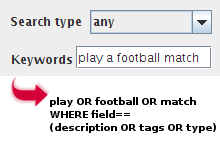
\includegraphics[scale=0.8]{screenshots/query-rich.png}
  \caption{\label{img:querying}Querying the search engine by using the GUI}
 \end{center}
\end{figure}

In the case of the search by similarity a deeper analysis was needed, but after
several tests, which will be detailed in Section \ref{sec:testing}, the queries
are composed by the following data of the application which is going to be
compared:
\begin{itemize}
  \item Application description.
  \item List of public tags.
  \item List of community tags associated to that application (which are visible
  for that user).
\end{itemize}

The query is composed in a similar way as in the one explained in Figure
\ref{img:querying}, and the search is performed on the fields ``description''
and ``tags'' for every application indexed by the search engine.


\subsection{Application adaptation}
\label{subsec:implementation-app-adaptation}
In this section we will explain the details related to the adaptation of an
application retrieved from the repository.
As it will be explained in Section \ref{sec:future-work}, this process aims to
have assistance by inferring using ontologies in the future.
The current state of the implementation performs some automatic changes, but it
still relies on the user's interaction.
\newline
On the other hand, the design and implementation have already taken into account
this possible expansion, so they are already connected with
\verb|OntologyManager| and call its services (which for the moment return a \verb|null| value) through its
interface. Since those methods are not implemented yet, 
\verb|ApplicationManager| offers the possibility of performing this process
manually as is shown in Figure \ref{img:manual-adaptation}.

\begin{figure}[h!]
 \begin{center}

 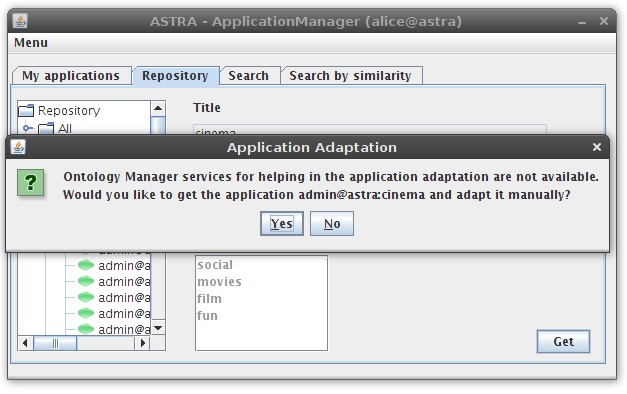
\includegraphics[scale=0.6]{screenshots/manual-adaptation-msg.png}
  \caption{\label{img:manual-adaptation}Offering the alternative of adapting the
  application manually (screenshot)}
 \end{center}
\end{figure}

We can divide the current adaptation functionalities offered in two sets: some
which are performed directly by the user and some that are performed
automatically in a transparent way.
\newline
As is shown in Figure \ref{img:application-adaptation}, the user can currently
modify the description of the application and select the rules before
retrieving the application.

\begin{figure}[h!]
 \begin{center}

 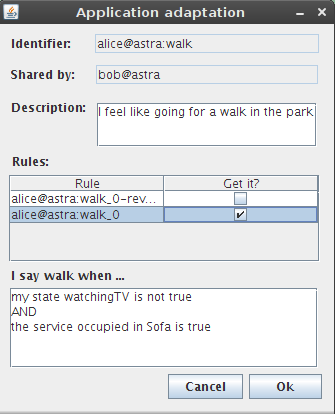
\includegraphics[scale=0.5]{screenshots/application-adaptation-retrieving.png}
  \caption{\label{img:application-adaptation}Application adaptation through the
  GUI (screenshot)}
 \end{center}
\end{figure}

The current automatic changes consist of changing the application and rules
identifiers (see Figure \ref{img:application-adaptation}) and changing
the rules ownership internally. The first one is almost straight, since it is
only necessary to reconstruct the Strings which identify the application or the
rule; but the internal changes in the rules require a deeper analysis.
\newline
The way in that we can access a rule is through an XML file which describes
it\footnote{This XML file is transformed to perform inference by
a subcomponent called \texttt{XMLToClipsParser}, but this is out of the scope of this
explanation.}.

An ASTRA XML rule has the following elements:
\begin{itemize}
  \item \verb|RULES|: The main rule tag that contains the rules. Each
  \verb|RULES| can contain more than one \verb|RULE|.
  \item \verb|RULE|: The tag that contains a single rule. Each rule needs a
  \verb|CONDITION| part and a \verb|RESULT| part.
   \item \verb|RULE_NAME|: The name of the rule.
   \item \verb|CONDITION|: The ``if part'' of the rule.
   \item \verb|TYPE|: The type of condition:
	\begin{itemize}
         \item If \verb|TYPE| is \verb|AND| or \verb|OR| type then it is
         followed by \verb|CONDITION_PART|.
         \item  If the \verb|TYPE| is Service, Awareness or InvokeMessage
         then it is followed by \verb|NAME|, \verb|OPERATOR| and \verb|VALUE|.
    \end{itemize}

   \item \verb|CONDITION_PART|: Defines the parts of a complex condition of an
   \verb|AND| or \verb|OR| type. It always contains two \verb|CONDITION| tags
   that define the two nested conditions.
  \item \verb|NAME|: The name of the variable for the condition.
	\begin{itemize}
      \item  If the \verb|TYPE| is Service, the notation is 
      \verb|<device>@<service>| where the \verb|<device>| is the device that 
      has the \verb|<service>|.
      \item If the \verb|TYPE| is Awareness, it is an intermediate state that 
      is usually described in the Awareness Ontology.
      \item If the \verb|TYPE| is InvokeMessage, it is the name of the
      application that we want to trigger.
    \end{itemize}
  \item \verb|OPERATOR|: The operator that describes the relationship between
	the \verb|NAME| and the \verb|VALUE|. Can be ``eq'', ``neq'', ``gt'', ``ge'',
	``lt'', ``le''. It can be omitted, in which case the default value is ``eq''.
   \item  \verb|VALUE|: The value that is compared with the \verb|NAME| in
   order to validate the condition.
  \item \verb|RESULT|: The ``then part'' of the condition. It is formed in the same
  way as a condition except that no operator is needed.
\end{itemize}


The Figure \ref{img:rule-internal-adaptation} shows an example of a simple XML
rule shared in the repository by user A (Alice), and the same XML rule after
applying the required changes in the ownership once user B (Bob) has retrieved
it. In general, this changes affect:

\begin{figure}[h!]
 \begin{center}

 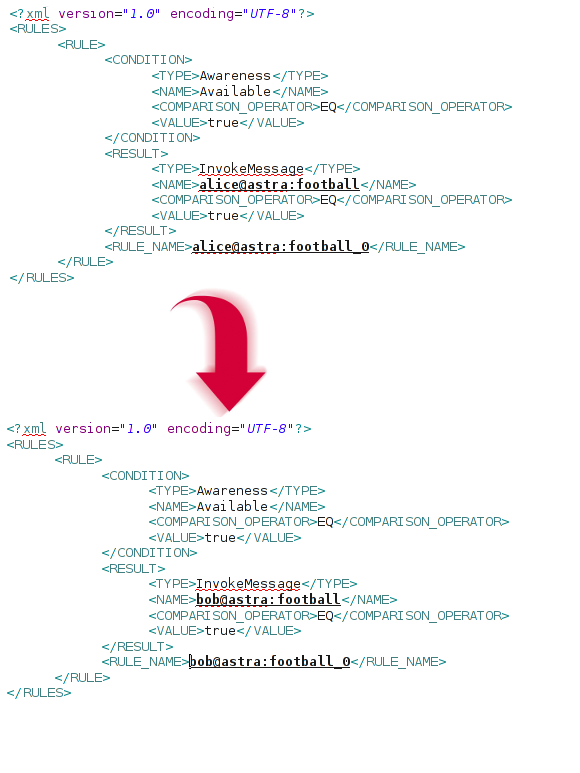
\includegraphics[scale=0.5]{screenshots/rules-transformation.png}
  \caption{\label{img:rule-internal-adaptation}Changes in the internal ownership
  of the rule}
 \end{center}
\end{figure}

\begin{itemize}
  \item All the nodes \verb|NAME| that are children of
  \verb|RESULT|.
  \item The node \verb|RULE_NAME|.
\end{itemize}

A similar approach was taken to create a description  of the rule based on
the XML file (as the one shown in Figure \ref{img:application-adaptation}) in
order to help the user to decide which rules he wants to appropriate. The Figure
\ref{img:rule-tree} shows graphically the way in which we create a human
readable description from a rule while analyzing recursively the
tree which represents the XML rule for an application (i.e.:
\verb|"bob@astra:walk"|).
%\footnote{Some of the nodes that are needed for the construction of the
%description (OPERATOR, VALUE, etc.) are omitted in Figure \ref{img:rule-tree}
%for simplicity reasons.}.

\begin{figure}[h!]
 \begin{center}
 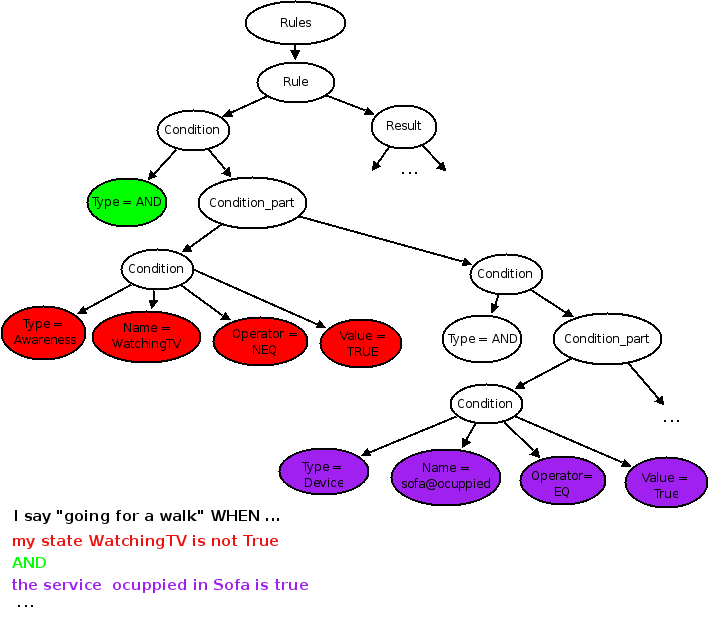
\includegraphics[scale=0.5]{diagrams/rule-tree.png}
  \caption{\label{img:rule-tree} Creating a rule description from an XML
  file}
 \end{center}
\end{figure}

This was implemented using DOM (see Section \ref{subsec:tech-dom}) in the
\verb|RepositoryManager|, and it is accessible for the rest of the bundles by
calling the method \verb|getXMLRule()| and \verb|getRuleDescription()| respectively.





